%! TeX program = pdflatex
\documentclass{article}
\usepackage[english]{babel}
\usepackage[utf8]{inputenc}
\usepackage{amsmath}
\usepackage{amssymb}
\usepackage{graphicx}
% \usepackage{natbib}
\usepackage{pgf}
% \usepackage{url}
\usepackage{algorithm}% http://ctan.org/pkg/algorithms
\usepackage{algpseudocode}% http://ctan.org/pkg/algorithmicx
% \usepackage{tikz-cd}
\usepackage{listings}
% \usepackage{xcolor}
% \usepackage[colorlinks, linkcolor = blue, citecolor = magenta]{hyperref}
\usepackage{tikz}
% % \usepackage{minted}
\usepackage{float}
% \usetikzlibrary{shapes, arrows, positioning}
% \lstset{ 
%     language=Python,                 % the language of the code
%     basicstyle=\ttfamily\small,      % the size of the fonts that are used for the code
%     numbers=left,                    % where to put the line-numbers
%     numberstyle=\tiny\color{gray},   % the style that is used for the line-numbers
%     stepnumber=1,                    % the step between two line-numbers. If it's 1, each line will be numbered
%     numbersep=5pt,                   % how far the line-numbers are from the code
%     backgroundcolor=\color{white},   % choose the background color. You must add \usepackage{color}
%     showspaces=false,                % show spaces adding particular underscores
%     showstringspaces=false,          % underline spaces within strings
%     showtabs=false,                  % show tabs within strings adding particular underscores
%     frame=single,                    % adds a frame around the code
%     rulecolor=\color{black},         % if not rolframe-color may be changed on line-breaks within not black text (e.g. comments (green here))
%     tabsize=4,                       % sets default tabsize to 4 spaces
%     captionpos=b,                    % sets the caption-position to bottom
%     breaklines=true,                 % sets automatic line breaking
%     breakatwhitespace=false,         % sets if automatic breaks should only happen at whitespace
%     title=\lstname,                  % show the filename of files included with \lstinputlisting; also try caption instead of title
%     keywordstyle=\color{blue},       % keyword style
%     commentstyle=\color{green},      % comment style
%     stringstyle=\color{red},         % string literal style
%     escapeinside={\%*}{*)},          % if you want to add LaTeX within your code
%     morekeywords={*,...} 
% }            % if you want to add more keywords to the rol\newenvironment{notation}
\newtheorem{remark}{Remark}
\newtheorem{definition}{Definition}
\newtheorem{property}{Property}

\newcommand{\pder}[2]{\frac{\partial #1}{\partial #2}}

\title{Electrical grid simulation in the COLMENA framework}
\author{Pablo de Juan Vela $^{1}$ \\
        \small $^{1}$eRoots, Barcelona, Spain \\
}
\date{\today}

\usepackage[style=ieee]{biblatex}
\addbibresource{ref.bib}
\setlength{\parskip}{1em} 
\begin{document}
\maketitle

\section{Introduction}
% ANDES intro
ANDES Curent \cite{grids:models} is a python package that can be used to model, simulate, and analyze power systems. The package uses predefined models that simulate different elements of an electrical grid. Additionally, the package allows the user to define custom models which relative ease. ANDES stands out from other simulation tools for the use of a hybrid symbolic-numeric framework for modeling differential algebraic equations (DAEs). This project present the objectives for developing test case for the COLMENA framework in the context of electrical grids using the simulation tools provided by ANDES. The goal of the project is to showcase the capabilities of COLMENA in the context of a decentralized electrical grid. We will outline the different requirements needed 

\subsection{Power Grid \& Service definition}
We define an electrical grid as a set of nodes called buses with electrical devices attached to them, the nodes are interconnected with lines. These devices include generators, loads or others types of devices. In ANDES, each device is defined by a set of differential and algebraic equations (DAE) that define how the devices' states change over time.
\vspace{1em} 
The electrical grid is defined by multiple metrics that define the state of the grid. Some of the more critical metrics that we consider are the following.

\begin{itemize}
    \item Frequency: The frequency is a local metric that describes the voltage at a specific bus. A device called Phasor Measurement Unit (PMU) can measure the frequency of the bus it is connected to. Maintaining the frequency at the nominal value of $50 Hz$ is key for the proper functioning of the grid. Values of the frequency above or below this value can unbalance the grid from a power point of view or even damage certain components.   
    \item Synchronous Rotor's Speed: Synchronous generators are device that generate power and then inject to the grid. This is done by spinning a rotor that spins at a certain speed, ideally as close as to the nominal frequency. The value of the frequency in the grids buses and the angular speed of the rotor are closely linked and are frequently used interchangeably. In fact, generators can see a drop in their angular speed to mitigate a drop in frequency in a close bus.
    \item Voltage $(V)$: The voltage is a metric linked to a specific bus and also needs to be as close to the nominal value as possible. Drops in frequency can be linked to drops in voltage.
    \item Power injected/consumed $(kW)$: The power injected is by a generator is the amount of power the . The objective of the grid supervisor is to keep the balance of power as close to zero as possible. Raising the amount of power injected by a generator also tends to raise its synchronous speed. It's an important lever in controlling  
\end{itemize}

The metrics just introduced are key to defining the performance of a grid and to the frequency control response of a power grid. The objective of the frequency response is multiple. On a first time scale (primary response)\cite{source:NRELfrequency}, the control aims to take the system from a transient to a stable condition and avoiding critical values for the frequency. During the secondary response, the objective is to restore the steady state values to their nominal values. Finally, the last response's objective is to restore the the power reserves to their original value \cite{source:bookelectron}.
\vspace{1em} 
The objective of the service implemented in COLMENA will be then to aid to the frequency control response by implementing decentralized roles that can improve the performance of the control. This roles will take the form of changing set-points for certain devices, connecting or disconnecting devices such as secondary generators and others. 

\subsection{ANDES' Devices}

A simulation created by the ANDES packages is organized around devices. Each device at a given time $t$ is defined by the value's of the algebraic variables and state variables. Devices of the same type have the same variables. Buses are one of the building blocks of the grid modeling. Other type of devices will connect to these buses. In the context of the frequency service control we have found the following devices that can be useful to the simulation and also present some sort of decentralized control.

\begin{itemize}
    \item Synchronous Generators: They inject power to the grid.
    \item Converters \& distributed generations: Used to convert power from distributed generation from DC to AC, usually associated to some sort of distributed generation.
    \item Loads: They consume power from the grid.
    \item Lines: They connect different buses.
    \item Switches: They allow the flow of power through a Line.
\end{itemize}

In the following sections we will se how these devices fit with the service of controlling the frequency.

\subsubsection*{Synchronous Generators}

Generators are devices that inject power to the grid. A synchronous generator injects the power through a rotating part that spins synchronously to the grid's frequency. The synchronous generators in the simulation will be defined by two internal states: $\omega \in \mathbb{R}$ the angular velocity and $\theta  \in \mathbb{R}$. The generator's turbine can set the value of the power being generator's or the set point for the reference angular speed $\omega_{ref}$. Controlling these set points is key to improve the performance of the grid.

\subsubsection*{Converters \& distributed generation}

The modelling of distributed generation in ANDES usually combines the generation considered as a DC current source and a battery that is connected to a AC-DC converter. The converter that is paired to this ensemble can control both the active and reactive power that is injected to the grid and that is stored in the battery (if present). The control of the setup is defined by the parameters $\gamma_p, \gamma_q \in [0,1]$ . These parameters define which proportion of the active and reactive power respectively and generated by the setup is injected to the grid. We can therefore define different operating points for the distributed generation depending on the power injected. The power that is not injected is then saved by the battery. This can be expressed as these three different operating points:

\begin{itemize}
    \item $\gamma_p = 1$ all of the power generated is injected to the grid.
    \item $\gamma_p = 0$ all of the power generated is stored in the battery.
    \item $\gamma_p = 0.5$ half of the power generated is injected to the grid and half is stored in the battery.
\end{itemize}


In the setup that we just explained the converter can take the form of a Voltage Source Converter (VSC). A VSC is a converter (converts a DC current to AC) with some differences to classical converters. They are commonly used to track the angle of the grid at a bus and inject (or absorb) active and reactive power from an energy source. They are usually paired with DC sources of energy as a way to connect them to the grid. We consider a VSC that can operate in two modes: 'Grid following'(GFL) and 'Grid forming'(GFM). 

\begin{itemize}
    \item Grid Following: In the GFL mode, the converter tracks the grid's frequency and injects a controlled power, acting as an ideal current source.
    \item Grid Forming: In the GFM mode, the converter creates its own frequency and imposes a voltage differential acting as an ideal voltage source.
\end{itemize}

In terms of control, both GFM and GFL have a reference value with a control. The control of the devices aims to get as close to the reference value as possible. For the GFL mode the reference value usually refers to the power injected, while for the GFM its the frequency or voltage. This GFM behavior is quite close to one of a typical synchronous generator. The flexibility and the different set points of this type of converter is fits well with the decentralized control principle of COLMENA.  

\subsubsection*{Loads}

A load is an electrical model that is connected to a bus and consumes a given amount of active and reactive($P(MW),  Q (Mvar)$ respectively). In the context of the frequency control service, the load device can have varying values of $P$ and $Q$ depending on the state of the grid. More specifically, . These adaptable response can be very useful to the grid in order to adapt to drops in generation or line faults.

\subsubsection*{Switches}
Switches are controllable elements that control the connection state of a Line. In this case the operating states are just 'Open' or 'Closed'. In the open state no current travels directly between the buses while in the Closed state the line works at normal operation. \\

\subsection{Andes-COLMENA Integration requirements}

In this section we explain how Andes and COLMENA will work during the simulation and how they will communicate. As a standalone, ANDES simulates the time domain response of the power grid for a pre-set amount of time. The package solves the equations numerically and return the solution but it doesn't simulate the grid in real time, instead it solves it as fast as possible. To enable the integration with COLMENA we modify ANDES into running for a given step-size only when the real time is greater than the simulation time in order for it to catch-up to. ANDES is run parallel to COLMENA on an independent app run on an independent device not part of COLMENA's colony of agents. Specific COLMENA Agents will periodically send requests to the ANDES App to get the simulation's information and to send changes   

From COLMENA's side, we will define specific COLMENA-agents that will be paired with a single ANDES-device in the grid. The COLMENA-agent will have two main roles in a continuous manner. They will read their device's variables, store the values internally, and send the behavior changes in the form of new set-point and parameter changes for the paired device. These roles will be the building blocks of the COLMENA-ANDES integration.      

\section{Use Case Specification}

Having explained the objectives of the project we want to chose specific scenarios that are well adapted to these objectives. In this particular case, we are looking for power grids of considerable size, and with the appropriate types of devices presented earlier such as generators, converters and distributed generation. Additionally, we would want to chose use cases in which the grid can be separated into different areas to properly implement into the simulation the different geographical context that we want to take into account. Finally, we also consider the ease to access information and data about the modeled grid.  

For the first use case we proposes first using the grid defined in  the Kundur two area system  \cite{grids:kundur}. This grid consists of 10 buses divided in 2 areas. Each area includes two synchronous generators. Additionally, this simulation includes a line failure at a specific time step (Line 8, at $t=2s$). The objective of this is to showcase how the decentralized nature of COLMENA can adapt to unexpected events in the grid such as failures and avoid cascading failures in the grid. 

\begin{figure}[!htb]
    \centering
    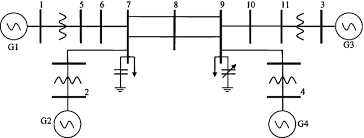
\includegraphics[width=0.5\textwidth]{pictures/kundurgrid.png}
    \caption{Kundur grid scheme. \cite{grids:kundur}}
    \label{fig:kundur2}
\end{figure}

In this specific use case the COLMENA-Agents will be paired with the different generators and monitor the values provided by the ANDES simulation. Moreover, this agents will be able to modify some of the generators values such as the power injected or internal controlling parameters. The objective is to overtime include different sources of generation and the proposed GFL-GFM converters. Let's see a proof of concept of what the integration could look like. In this use case one of the COLMENA Agents is able to modify the inertia parameter of the generator 1 inside the simulation depending of the value of the generator's speed $\omega$. By modifying the inertia what we expect to see is the generator's angular velocity $\omega$ having 2 distinct behaviors.  

\begin{table}[H]
    \centering
    \begin{tabular}{|l|l|l|}
    \hline
    Operating State & KPI                              & Parameter $M$ value \\ \hline
    A               & $\omega \in [1 - \varepsilon, 1 + \varepsilon]$ & 12  \\ \hline
    B               & $\omega \notin [1 - \varepsilon, 1 + \varepsilon]$ & 120               \\ \hline
    \end{tabular}
    \caption{Generator set-points summary.}
\end{table}
  

\begin{figure}[h]  % [h] places the figure "here"
    \centering
    % Fit the PGF figure to the page width
    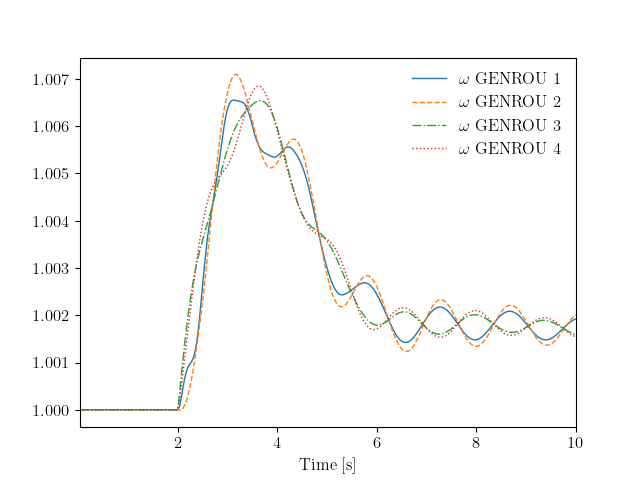
\includegraphics[width=1\textwidth]{pictures/plot.png}

    \caption{Time series of the distributed generator's frequency.}
    \label{fig:sample_figure2}
\end{figure}

When this more accessible use case is deploy we want to scale the simulation into a more extensive grid that could be able to showcase the performance of COLMENA in a more complicated environment, with more varieties of models and more complicated control overall. The objective is to eventually run the simulation in larger grids with a larger number of agents. For this we can use other test grids such as the IEEE 118 bus case \cite{grids:ieee118}. This test grid is composed by 118 buses, 54 generators and 99 Loads. Additionally, some of the generators are synchronous condensers who essentially are synchronous motors whose shaft is not connected to any mechanical load. Their main function is to provide reactive power compensation. Moreover, it uses the same models as the ones used in the previous tests cases so transferring the already developed models is feasible.

\begin{figure}[h!]
    \centering
    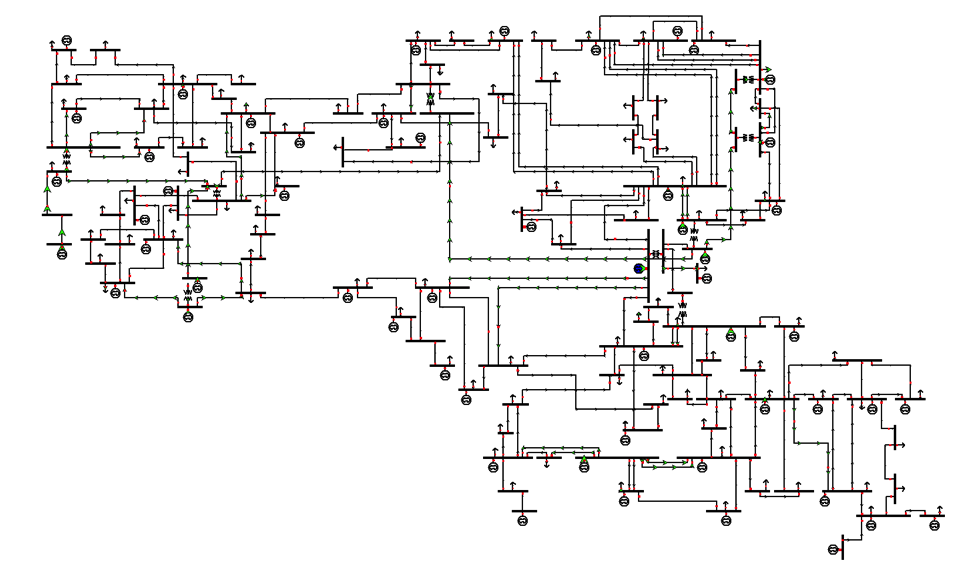
\includegraphics[width=1\textwidth]{pictures/IEEE118.png}
    \caption{IEEE118 grid scheme. \cite{grids:ieee118}}
    \label{fig:kundur}
\end{figure}

\subsection{Grid's Performance \& Key Performance Indicators}

In the first section we have defined a set of metrics and states that are key to defining the grids state, specifically when dealing with the frequency response. These include the frequency, the angular speed of the synchronous generators and others. We aim to define key performance indicators (KPI) starting from the metrics defined previously. These KPIs define the performance of the grid with respect to the frequency service control. 

\begin{itemize}
    \item Minimum and maximum of the generator's frequency.
    \item Minimum and maximum of the mean bus frequency in an area from the nominal frequency.
    \item Steady state values.
    \item Rate of Change of Frequency (RoCoF).
    \item Available power reserves.
    \item Power Balance \& regional power exchanges.
    \item N-1 criteria
    \item Economic criteria
\end{itemize}

\subsection*{Minimum and maximum of the generator's frequency}

This KPIs is usually used with regards to the primary response in the frequency control response. The objective would be to maintain the generator's frequency $\omega$ as close to the nominal value. In power grids a common value for this KPI in the response is around $0.1\%$ around the nominal value. This is true for both the generator's frequency and the buses' frequency.

\subsection*{RoCoF}

The Rate of Change of Frequency is the frequency's time derivative measured in a given bus. It signals sudden changes in frequency and if its close to $0$ for a given amount of time it can also signal the grid arriving to a steady state. Therefore the RoCoF is key to measure the performance of the grid during. 

\subsection*{Available Power Reserves}

The available power reserves is the amount of power that can be activated in a given amount of time in case of need but its not being used. It usually considers an horizon of 10 to 30 minutes. Additionally, we also need to consider the ramp up capabilities of these power reserves. The ramp up measured in kW/s and is the speed with which this reserve power can come online. The grid operator usually defines minimum requirements for available power values.

\subsection*{Maximum line current}

The current through a line is limited by a maximum value for security purposes. If the current through a line surpasses the maximum value for a specific amount of time the line can disconnect to avoid being damaged.

\subsection*{Power Balance \& regional power exchanges}

The power balance is defined as the net power that is coming into the grid. A good performance of the grid should maintain the net power balance close to 0. Additionally, we can also look into the power balances between different areas that are interconnected and define KPI that take into account excessive reliance on these interconnections. One KPI that could be useful for taking into account these power exchanges between areas is the Area Control Error (ACE). The ACE of an area is defined as the difference between the net power exchange and the schedule power exchange with all adjacent areas. It measures if the grid is sticking to the scheduled power exchanges. A good performing grid looks to have an ACE close to $0$.  

\subsection*{N-1 criteria}

The N-1 criterion is a standard used in power system planning and operation to ensure reliability and resilience. It specifies that a power system should be able to withstand the loss of any single element (like a generator, transformer, or transmission line) without causing a system-wide failure. New devices could be connected or scheduled by the COLMENA agents to help ensure the criterion is respected. 


\subsection*{Economic criteria}


\nocite{*}
\printbibliography
\end{document}